\section[تمرین دوم: پیش‌بینی بارش (\lr{BOM Dataset})]{\faCloudRain\ \ تمرین دوم: پیش‌بینی بارش با KNN}

\begin{stepbox}

\field{پیش‌پردازش داده‌ها (\lr{Preprocessing})}{
مراحل پیش‌پردازش روی مجموعه داده \lr{BOM} به صورت یکپارچه با ابزار \lr{Pipeline} پیاده‌سازی شد:
\begin{itemize}
    \item \textbf{رمزگذاری ویژگی‌های چرخه‌ای:} استخراج ماه و روزِ هفته از تاریخ و همچنین جهت وزش باد، و تبدیل آن‌ها به مولفه‌های سینوسی و کسینوسی برای حفظ کامل خاصیت دوره‌ای زمان و جهت.
    \item \textbf{استخراج ویژگی‌های مکانی:} جایگزینی نام متنی شهرها با مختصات جغرافیایی دقیق طول و عرض (\lr{Latitude / Longitude}).
    \item \textbf{مدیریت داده‌های گمشده (\lr{Imputation}):} متغیرها بر اساس درصدِ مقادیر ازدست‌رفته گروه‌بندی شدند:
    برای کمتر از $5\%$ از میانه، بین $5\%$ تا $30\%$ از الگوریتم \lr{KNNImputer} (با $k=5$)، و برای مقادیر بیش از $30\%$ از میانه به همراه یک متغیر نشانگر (\lr{Indicator}) استفاده شد.
\end{itemize}
}

\field{آموزش مدل و تنظیم پارامترها}{
الگوریتم \lr{K-Nearest Neighbors} روی داده‌های مقیاس‌شده با \lr{StandardScaler} برای مقادیر مختلف $k \in \{1, 2, 3, 5, 9, 15, 21, 31\}$ ارزیابی شد. برای افزایش سرعت اجرا و بهینه‌سازی محاسباتی، فواصل یک‌بار برای ماکزیمم مقدار $k$ محاسبه گردید.

\vspace{0.4cm}
\begin{center}
    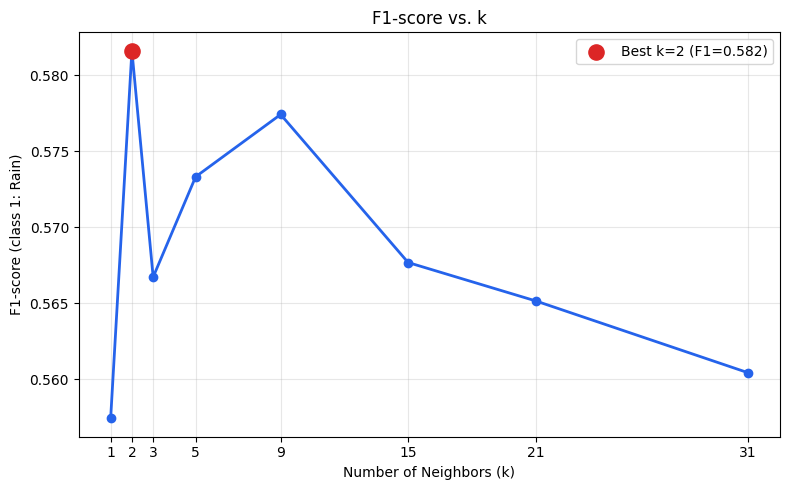
\includegraphics[width=0.5\textwidth]{images/knn_f1.png}
    \captionsetup{hypcap=false}
    \captionof{figure}{تغییرات معیار $\mathit{F1}\text{-score}$ به ازای مقادیر مختلف $k$. بهترین عملکرد در $k=2$ با امتیاز $0.582$ حاصل شده است.}
    \label{fig:knn_k_plot}
\end{center}
}

\field{تحلیل عملکرد مدل بر اساس نمودار}{
همان‌طور که در نمودار \ref{fig:knn_k_plot} مشخص است، مدل با $k=2$ بالاترین معیار \lr{F1-score} را برای تشخیص کلاس هدف (بارش) ثبت کرده است. مقادیر بالاتر $k$ به دلیل افزایش نرمی مرزهای تصمیم‌گیری، باعث افت شدید حساسیت مدل (\lr{Recall}) در شناسایی کلاس اقلیت شده‌اند.
}

\field{پاسخ به سوال تحلیلی (سیستم‌های بلادرنگ)}{
\textbf{سوال:} برای یک سیستم پیش‌بینی بلادرنگ (\lr{Real-time})، کدام الگوریتم انتخاب بهتری است؟ \\
\textbf{پاسخ:} الگوریتم \textbf{درخت تصمیم (\lr{Decision Tree})} انتخاب بسیار بهتری نسبت به \lr{KNN} است.
دلیل این امر این است که \lr{KNN} یک یادگیرنده تنبل (\lr{Lazy Learner}) است و در فاز تست (آزمون)، باید فاصله داده جدید را با تک‌تک نمونه‌های آموزشی محاسبه کند که زمان اجرای آن متناسب با پیچیدگی زیر است و به‌شدت کند می‌شود:
\[ \mathcal{O}(n \times d) \]

در مقابل، درخت تصمیم یک یادگیرنده مشتاق (\lr{Eager Learner}) است و پس از آموزش، زمان پیش‌بینی آن تنها متناسب با عمق درخت بوده و از مرتبه بسیار سریع زیر خواهد بود که سرعت فوق‌العاده بالایی در سیستم‌های عملیاتی دارد:
\[ \mathcal{O}(\log n) \]
}

\end{stepbox}